% LaTeX source for ``การเรียนรู้ของเครื่องสำหรับเคมีควอนตัม (Machine Learning for Quantum Chemistry)''
% Copyright (c) 2022 รังสิมันต์ เกษแก้ว (Rangsiman Ketkaew).

% License: Creative Commons Attribution-NonCommercial-NoDerivatives 4.0 International (CC BY-NC-ND 4.0)
% https://creativecommons.org/licenses/by-nc-nd/4.0/

\chapter{คุณสมบัติเชิงอิเล็กทรอนิกส์ของโมเลกุล}
\label{ch:el_prop}

\begin{figure}[htbp]
    \centering
    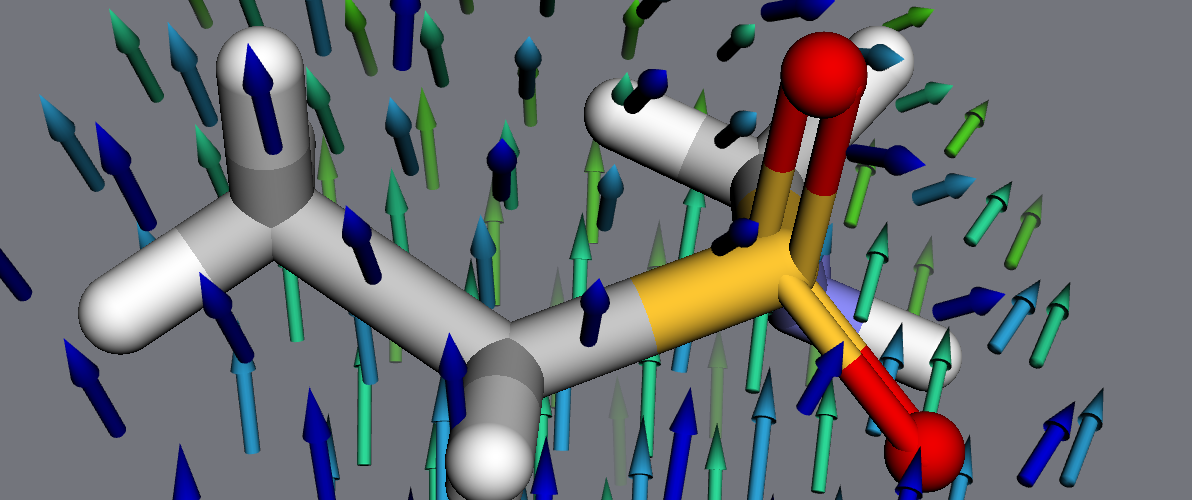
\includegraphics[width=0.9\linewidth]{fig/mol_properties.png}
    \caption{สนามเวกเตอร์ของโมเลกุลเมื่ออยู่ในสนามแม่เหล็ก}
    \label{fig:mol_prop}
\end{figure}

เนื้อหาในบทนี้จะต่อเนื่องจากบทที่ \ref{ch:el_strct} โดยเราจะมาดูรายละเอียดของทฤษฎีของคุณสมบัติเชิงอิเล็กทรอนิกส์ (Electronic 
Properties) ของโมเลกุลแบบต่าง ๆ ซึ่งผู้เขียนคิดว่าเป็นสิ่งที่สำคัญมากนั่นก็เพราะว่าถ้าหากเราต้องการที่จะเชื่อมโยง ML และเคมีควอนตัมเข้า%
ด้วยกันเราควรจะต้องเข้าใจถึงทฤษฎีของคุณสมบัติของโมเลกุลที่เราต้องการที่จะศึกษาเสียก่อน เมื่อเราเข้าใจทฤษฎีแล้วก็จะทำให้เกิดไอเดียที่เรา%
สามารถประยุกต์ใช้ ML ได้อย่างถูกต้อง

%--------------------------
\section{ความหนาแน่นเชิงประจุและเมทริกซ์ความหนาแน่น}
\label{sec:charge_den}
\idxboth{ความหนาแน่นเชิงประจุ}{Charge Density}
%--------------------------

ความหนาแน่นเชิงประจุ (Charge Density) เป็นปริมาณที่บ่งบอกถึงประจุของอะตอมที่อยู่ในโมเลกุล ถ้าหากเราทำการอินทิเกรต Charge Density 
ทั่วทั้งปริมาตรเราจะได้ผลลัพธ์เป็นจำนวนของอิเล็กตรอนในระบบของเรา (โมเลกุล) ดังนี้\autocite{szabo1996}

\begin{equation}
    N = \int \rho(\bm{r}) dV
\end{equation}

โดยนิยามของ Charge Density จะเป็นผลรวมของโอกาสที่เราจะพบอิเล็กตรอนที่อยู่ภายใน Molecular Orbitals ของทั้งระบบ ดังนี้
\idxen{Charge Density}

\begin{equation}\label{eq:charge_density}
    \rho(\bm{r}) = 2 \sum^{N/2}_{i=1} \int |\varphi_{i}(\bm{r})|^{2}
\end{equation}

\noindent โดยเลข 2 ด้านหน้าเครื่องหมาย Summation ก็คือ Occupation Number สำหรับกรณีที่ Molecular Orbital $(i)$ 
นั้นมีอิเล็กตรอนทั้งแบบ Spin Up และ Spin Down และ $\varphi_{i}(\bm{r})$ คือ Wavefunction ซึ่งเราสามารถเขียน Wavefunction 
ให้อยู่ในรูปผลรวมเชิงเส้น (LCAO) ของ Basis Function $(\phi_{i})$ ซึ่ง Basis Function นี้จะเป็นฟังก์ชันอะไรก็ได้ที่สามารถอธิบายการ%
มีอยู่ของ Molecular Orbital โดยในกรณีแบบที่ง่ายที่สุดคือเราจะมองว่า Molecular Orbital นั้นเกิดขึ้นจากการรวมกันของ Atomic Orbitals 
ดังนั้นเราจะกำหนดให้ Atomic Orbitals เป็น Basis Function\footnote{Basis Function ในที่นี้คือ Atomic Orbitals ที่ถูกกำหนดให้%
มีจุดศูนย์กลางอยู่ที่อะตอมนั้น ๆ} ดังนั้นเราสามารถเขียน LCAO ได้ดังต่อไปนี้ 
ตามสมการดังต่อไปนี้
\idxen{Basis Function}

\begin{equation}
    \rho(\bm{r}) = 2 \sum_{i} \left ( \sum_{\mu} c_{\mu i} \phi_{\mu}^{*} \right ) 
    \left ( \sum_{\nu} c^{*}_{\nu i}  \phi_{\nu} \right )
\end{equation}

\noindent โดยที่ $c$ คือสัมประสิทธิ์ของ LCAO ลำดับต่อมาคือเมื่อเราจัดรูปให้มีเทอมที่เป็นผลคูณของ Basis Function $(\phi_{\mu}^{*} 
\phi_{\nu})$ เราจะกำหนดให้เทอมนี้เป็นสิ่งที่เรียกว่าเมทริกซ์ซ้อนทับ (Overlap Matrix) หรือ $S_{\mu\nu}$ โดยจะได้สมการที่จัดรูปแล้ว 
ดังนี้
\idxboth{เมทริกซ์ซ้อนทับ}{Overlap Matrix}

\begin{equation}
    \rho(\bm{r}) = 2 \sum_{i}\sum_{\mu\nu} c_{\mu i} c^{*}_{\nu i} S_{\mu\nu}
\end{equation}

หลังจากนั้นเราจะพบว่าจะมีเทอมที่เป็นผลคูณระหว่าง $c$ ซึ่งเราเรียกผลคูณแบบนี้ว่าเมทริกซ์ความหนาแน่น (Density Matrix) 
\idxboth{เมทริกซ์ความหนาแน่น}{Density Matrix}

\begin{equation}\label{eq:density_matrix}
    P_{\mu\nu} = c_{\mu i} c^{*}_{\nu i}
\end{equation}

\noindent ซึ่งเราจะได้สมการของความหนาแน่นเชิงประจุในรูปของเมทริกซ์ความหนาแน่นดังต่อไปนี้

\begin{equation}\label{eq:charge_density_matrix}
    \rho(\bm{r}) = 2 \sum_{i} \sum_{\mu\nu} P_{\mu\nu}S_{\mu\nu}
\end{equation}

%--------------------------
\section{ประจุย่อย}
\label{sec:partial_charge}
\idxboth{ประจุย่อย}{Partial Charge}
\idxboth{ประจุเชิงอะตอม}{Atomic Charge}
%--------------------------

การวิเคราะห์ Wavefunction หลังจากการคำนวณเป็นสิ่งที่สำคัญมากเพราะจะช่วยให้เราเข้าใจถึงพฤติกรรมเชิงอิเล็กทรอนิกส์ของอะตอมภายในโมเลกุล 
โดยหนึ่งในคุณสมบัติเชิงอิเล็กทรอนิกส์ที่นักเคมีทฤษฎีมักจะทำการวิเคราะห์เป็นอันดับแรกเสมอ (นอกจากพลังงานเชิงอิเล็กทรอนิกส์) นั้นก็คือประจุย่อย%
ของแต่ละอะตอม (Partial Atomic Charge) ซึ่งมีความสำคัญมากเพราะว่าถ้าหากเราทราบค่าประจุย่อยของอะตอมในโมเลกุลจะช่วยทำให้สามารถ%
เข้าใจว่าอะตอมแต่ละตัวส่งผลหรือมี Contribution มากน้อยเพียงใดเมื่อเทียบกับอะตอมอื่น ๆ ภายในโมเลกุลเดียวกัน

ต้องอธิบายก่อนว่าประจุรวมของโมเลกุลเกิดจากผลรวมของประจุย่อยของอะตอมแต่ละตัว (Partial Atomic Charge) ซึ่งในทางทฤษฎีและการทดลอง%
เราไม่มีนิยามที่แน่นอนในการระบุหรือกำหนดประจุย่อยของอะตอมแต่ละตัวในโมเลกุล อย่างไรก็ตามได้มีทฤษฎีต่าง ๆ มากมายที่ถูกเสนอและพัฒนามาเพื่อ%
ใช้ในการคำนวณประจุย่อย โดยแนวคิดแรก ๆ ก็ได้ถูกพัฒนามานานหลายสิบปีแล้ว หนึ่งในนั้นก็คือทฤษฎีที่ตั้งอยู่บนแนวคิดพื้นฐานของ Wavefunction 
ซึ่งใช้ Population ของ Atomic Orbital (Basis Set) เช่น Mulliken Population ที่เราสามารถนำมาใช้ในการคำนวณประจุอะตอม 
เรียกว่าประจุของมัลลิเคน (Mulliken Charge) ซึ่งออร์บิทัลของอะตอมที่อยู่ในโมเลกุลถูกกำหนดและแบ่งด้วยเมทริกซ์ซ้อนทับ (Overlap Matrix) 
เนื่องจากว่าประจุย่อยเป็นปริมาณที่วัดไม่ได้ (Non-observable Property) กล่าวคือไม่สามารถวัดได้ในทางทดลอง นั่นก็เพราะว่าจริง ๆ แล้วโมเลกุล%
นั้นไม่ได้เกิดขึ้นจากที่อะตอมแต่ละตัวมาต่อติดกัน แต่ว่าเป็นกลุ่มก้อนอะตอมที่มารวมกันแบบราบเรียบ (Smooth) ดังนั้นเราจึงไม่สามารถที่จะระบุได้ว่า%
อะตอมแต่ละตัวนั้นมีขนาดเล็กหรือใหญ่แค่ไหน กล่าวคือเราไม่รู้ว่าอะตอมและตัวเริ่มต้นตรงไหนและสิ้นสุดตรงไหน นั่นจึงทำให้เราไม่รู้ขอบเขตของแต่ละ%
อะตอมนั่นเอง
\idxboth{เมทริกซ์ซ้อนทับ}{Overlap Matrix}

นอกจากนี้ยังมีอีกหลายทฤษฎี/วิธีที่ได้ถูกพัฒนาขึ้นมาเพื่อกำหนดนิยามของประจุย่อยของอะตอม ดังนี้

\begin{enumerate}
    \item วิธีที่ใช้ออร์บิทัล (Orbital-based) ซึ่งเป็นการทำ Population โดยใช้ Basis Functions
        \begin{enumerate}
            \item Mulliken Charge\autocite{szabo1996} เป็นวิธีที่ได้รับความนิยมเป็นอย่างมากสำหรับคำนวณประจุย่อยของอะตอมซึ่ง%
            โปรแกรมเคมีเชิงคำนวณหลาย ๆ โปรแกรมมักจะคำนวณ Mulliken Charge ให้โดยอัตโนมัตินั่นก็เพราะว่าสามารถคำนวณได้ง่าย%
            โดยใช้ Density Matrix $(P)$ และ Overlap Matrix $(S)$ ซึ่งได้จากการคำนวณโครงสร้างเชิงอิเล็กทรอนิกส์ ซึ่งวิธี 
            Mulliken นั้นจะเกี่ยวข้องกับการแบ่ง (Partition) ผลคูณระหว่าง $P$ และ $S$ ดังนี้

            \begin{equation}\label{eq:mulliken_pop}
                \rho_{A} = \sum^{M_{\text{basis}}}_{\alpha \in A} \sum^{M_{\text{basis}}}_{\beta}
                P_{\alpha\beta} S_{\alpha\beta}
            \end{equation}

            \noindent โดยที่ $\rho_{A}$ คือ Population ของอะตอม $A$ และ $\alpha$ และ $\beta$ คือออร์บิทัลเชิงอะตอม 
            (Atomic Orbitals, AOs) ซึ่งประจุของอะตอม $A$ นั้นสามารถหาจากได้ผลต่างจากเลขนิวเคลียร์ของอะตอม ดังนี้

            \begin{equation}\label{eq:mulliken_charge}
                Q_{A} = Z_{A} - \rho_{A}
            \end{equation}

            \noindent โดยการใช้ผลคูณ $\sum P \cdot S$ นั้นเป็นการกระจายอิเล็กตรอนให้อยู่ในรูปของการมีส่วมรวมเชิงอะตอม (Atomic 
            Contributions) นั่นเอง หมายความว่าสมาชิกแนวทแยง $P_{\alpha\alpha} S_{\alpha\alpha}$ นั้นเป็นจำนวนของอิเล็ก%
            ตรอนและสมาชิกนอกแนวทแยง $P_{\alpha\beta} S_{\alpha\beta}$ เป็นจำนวนครึ่งหนึ่งของจำนวนอิเล็กตรอนที่ถูกแชร์%
            ระหว่าง AOs $\alpha$ และ $\beta$
            
            \item L\"{o}wdin Charge\autocite{lowdin1950} วิธีต่อมาที่เปรียบเสมือนเป็นพี่น้องกับ Mulliken Charge นั่นก็คือประจุ
            L\"{o}wdin โดยจะเป็นเมทริกซ์ซ้อนทับแบบแบ่งส่วน (Partition Overlap Matrix) ดังนี้

            \begin{align}
                \sum P \cdot S &= N_{\text{elec}} \\
                \sum S^{\frac{1}{2}} \cdot (P \cdot S) \cdot S^{-\frac{1}{2}} &= 
                S^{\frac{1}{2}} N_{\text{elec}} S^{-\frac{1}{2}}\\
                \sum S^{\frac{1}{2}} \cdot D \cdot S^{\frac{1}{2}} &= N_{\text{elec}} \label{eq:lowdin_charge}
            \end{align}
        \end{enumerate}

        ถ้าหากผู้อ่านสังเกตดี ๆ จะพบว่าทั้งวิธี Mulliken และ L\"{o}wdin นั้นต่างก็เป็นเพียงแค่รูปแบบเฉพาะของการทำ Population Analysis 
        ที่ใช้ $S^{n} \cdot P \cdot S^{1-n}$ เท่านั้น โดยที่กรณีที่ $n=0$ นั้นก็จะเป็น Mulliken และกรณีที่ $n=\frac{1}{2}$ นั้นก็%
        จะเป็น L\"{o}wdin

        อย่างไรก็ตามไม่มีวิธีไหนนั้นดีที่สุด ถึงแม้ว่าการทำ Population Analysis โดยอ้างอิงกับ Basis Function นั้นจะง่ายแต่ก็มีปัญหา%
        อยู่หลายข้อด้วยกัน ดังนี้ 

        \begin{enumerate}[topsep=0pt]
            \item สมาชิกแนวทแยงของ Population สำหรับบางออร์บิทัลนั้นอาจจะมีค่ามากกว่า 2 ได้ ซึ่งขัดแย้งกับหลักการของเพาลี
            
            \item สมาชิกนอกแนวทแยงอาจจะมีค่าเป็นลบได้ ซึ่งบอกเป็นนัย ๆ ว่าจำนวนอิเล็กตรอนระหว่าง Basis Function นั้นเป็นลบด้วย%
            ซึ่งไม่มีทางเป็นไปได้

            \item เราไม่สามารถหาเหตุผลมาอธิบายได้ว่าเมื่อไหร่ควรจะใช้ Population Method แบบนี้เพราะว่าเราไม่รู้ว่าการที่เราแบ่งครึ่ง%
            ออร์บิทัลออกจากกันแบบเท่า ๆ กันนั้นจะสอดคล้องกับค่า Electronegativity ของอะตอมด้วยหรือไม่
        \end{enumerate}
    
    \item วิธีที่ใช้ศักย์เชิงไฟฟ้าสถิตย์ (Electrostatic Potential-based) \\
    
        เป็นวิธีที่ถูกพัฒนาโดยใช้หลักการระหว่างศักย์เชิงไฟฟ้าสถิตย์ (Electrostatic Potential หรือ ESP) กับอนุภาคที่มีประจุ โดย ESP
        ที่ตำแหน่ง $\bm{r}$ สามารถคำนวณได้จากผลรวมของ Contribution จากนิวเคลียสและความหนาแน่นของอิเล็กตรอน ดังนี้

        \begin{equation}\label{eq:esp_population}
            \phi_{\text{ESP}}(\bm{r}) = \sum^{\text{nuclei}}_{A} \frac{Z_{A}}{|\bm{r} - \bm{R}_{A}|} 
            - \int \frac{\rho(\bm{r}')}{|\bm{r} - \bm{r}'|} d\bm{r}'
        \end{equation}

        \noindent โดยที่ 
        
        \begin{equation}
            \rho(\bm{r}') = |\Psi(\bm{r}')|^{2}
        \end{equation}

        เทอมแรกของสมการที่ \ref{eq:esp_population} สามารถคำนวณได้อย่างง่าย ๆ จากประจุนิวเคลียร์และตำแหน่งของอะตอมแต่ว่า%
        เทอมที่สองของสมการซึ่งเป็นผลจากอิเล็กตรอนนั้นจำเป็นที่จะต้องใช้ Wavefunction เข้ามาช่วยซึ่งทำได้ไม่ง่าย นอกจากนี้แล้วเทอมที่%
        สองนั้นไม่ได้ถูกรวมเข้าไปในบางวิธี เช่น วิธี Force Field ที่ใช้ในการจำลองแบบ Molecular Dynamics ดังนั้นวิธีที่ง่ายที่สุดในการ%
        จำลองเทอมที่สองหรือ Electrostatic Potential นั้นก็คือการกำหนดค่าประจุย่อยให้แต่ละอะตอมโดยตรงเลย โดยพารามิเตอร์ของ 
        Force Field นั้นสามารถหาได้จากการ Fit ค่าเทียบกับข้อมูลเชิงการทดลอง เช่น Dipole Moment, Quadrupole Moment, 
        หรือ Octopole Moment

        นอกจากนี้แล้วยังมีวิธีอื่น ๆ อีกหลายวิธีในการกำหนด ESP สำหรับการคำนวณค่าประยุย่อยเชิงอะตอม โดยวิธีเหล่านั้นก็มีความแตกต่างกันที่%
        วิธีที่ใช้ในการกำหนดจำนวนและตำแหน่งของจุด (Point) ที่ใช้ในการสุ่มตัวอย่าง (Sampling) ESP โดยจำนวนจุดที่ใช้ในการ Sampling 
        นั้นมักจะอยู่ที่ประมาณหลักร้อยจุดรอบ ๆ นิวเคลียส โดยระยะห่างระหว่างจุดถึงนิวเคลียสนั้นมักจะถูกกำหนดให้ไม่เกินสองเท่าของรัศมี van 
        Der Waals สำหรับวิธีอื่น ๆ ของ ESP นั้นมีดังต่อไปนี้

        \begin{enumerate}
            \item Merz-Singh-Kollman (MSK) Charge\autocite{singh1984}
            
            \item Charges from the Electrostatic Potential (CHELP) Charge\autocite{chirlian1987}
            
            \item Charges from the Electrostatic Potential on a Grid (CHELPG) Charge\autocite{breneman1990}
            
            \item Restrained Electrostatic Potential (RESP)\autocite{cornell1993}
        \end{enumerate}
    
    \item วิธีที่ใช้ความหนาแน่นของอิเล็กตรอน (Electron Density-based)
    
    ในหัวข้อก่อนหน้านี้ผู้อ่านได้ศึกษาการหา Population โดยอ้างอิงกับ Wavefunction ไปแล้ว ในหัวข้อนี้จะเป็นการวิเคราะห์ Population 
    โดยใช้ความหนาแน่นของอิเล็กตรอน ซึ่งตามที่เราได้ศึกษาไปในหัวข้อ \ref{sec:dft} แล้วว่าความหนาแน่นของอิเล็กตรอนนั้นคือ Wave 
    Function ที่ถูกยกกำลังสองซึ่งถูกอินทิเกรตทั่วทั้ง Coordinate ของอิเล็กตรอนจำนวน $N_{\text{elec}} - 1$ โดยความยากในการแบ่ง%
    (Partitioning) ความหนาแน่นของอิเล็กตรอนให้เป็นผลรวมของการมีส่วนร่วมเชิงอะตอม (Atomic Contribution)%
    \footnote{ผู้เขียนแปลคำว่า Contribution เป็นการมีส่วมร่วมก็เพราะว่าเป็นการบ่งบอกว่าอะตอมแต่ละอะตอมนั้นส่งผลในเชิงอิเล็กทรอนิกส์%
    ต่อโมเลกุลเทียบกับอะตอมตัวอื่น ๆ มากน้อยแค่ไหน} นั้นคือขึ้นอยู่กับว่าเราจะกำหนดคำว่าอะตอมที่อยู่ภายในโมเลกุลอย่างไร ซึ่งตรงจุดนี้แหละ%
    ที่เป็นความยากเพราะว่าจริง ๆ แล้วรอยต่อระหว่างอะตอมนั้นมันราบเรียบและเราไม่สามารถหารอยต่อหรือขอบเขตที่ชัดเจนและแน่นอนได้ 

    ไอเดียก็คือถ้าหากว่าผลรวมของปริมาตรเชิงโมเลกุลนั้นสามารถถูกแบ่งออกเป็นปริมาตรส่วนย่อย ๆ ได้แล้วปริมาตรย่อย ๆ แต่ละส่วนนั้นก็เป็นส่วน%
    หนึ่งของนิวเคลียส เราจะสามารถอินทิเกรตความหนาแน่นของอิเล็กตรอนและคำนวณจำนวนของอิเล็กตรอนในรูปของเชิงอะตอมได้ $(\Omega)$ 
    แล้วสิ่งที่เราจะทำได้เพิ่มเติมก็คือประจุเชิงอะตอม $Q$ นั้นสามารถหาได้จากประจุเชิงนิวเคลียร์ $Z$ ดังนี้

    \begin{equation}\label{eq:N_elec}
        N_{A} = \int_{\Omega} \rho(\bm{r}) d\bm{r}
    \end{equation}

    \begin{equation}
        Q_{A} = Z_{A} - N_{A}
    \end{equation}

    \noindent โดยสมการที่ \ref{eq:N_elec} สามารถถูกทำให้อยู่ในรูปทั่วไป (Generalized) ได้ตามสมการดังต่อไปนี้
    
    \begin{equation}\label{eq:N_elec_general}
        N_{A} = \int_{\Omega} w_{A}\bm{r} \rho(\bm{r}) d\bm{r}
    \end{equation}

    \noindent โดยที่ $w_{A}(\bm{r})$ คือฟังก์ชันถ่วงน้ำหนักที่กำหนดค่าสัดส่วนของความหนาแน่นของอิเล็กตรอนที่ตำแหน่ง $\bm{r}$ 
    ที่ขึ้นอยู่กับอะตอม $A$

    นอกจากนี้ยังมีทฤษฎีเพิ่มเติมที่ได้มีการนำเสนอแนวคิดที่น่าสนใจเกี่ยวกับการแบ่งโมเลกุลออกเป็นอะตอม เช่น 

    \begin{enumerate}
        \item Hirshfeld Charge\autocite{hirshfeld1977}
        
        \item Atoms in Molecules (AIM) หรือ Bader Charge\autocite{bader1985,bader1991}
    \end{enumerate}
    
    \item เทนเซอร์เชิงขั้ว (Polar Tensor)\autocite{person1974,milani2010}
    
    อีกหนึ่งวิธีที่น่าสนใจที่ถูกพัฒนาขึ้นมาเพื่อคำนวณประจุย่อยเชิงอะตอมนั้นก็คือเทนเซอร์เชิงขั้วของอะตอม (Atomic Polar Tensor หรือ APT) 
    โดยถูกพิสูจน์มาจากอนุพันธ์ของ Dipole Moment เทียบกับตำแหน่งของนิวเคลียสซึ่งเป็นตัวที่กำหนดความเข้ม (Intensity) ของการดูดกลืน%
    แบบ Infrared โดยสมการสำหรับการคำนวณประจุ APT นั้นมีดังต่อไปนี้

    \begin{equation}\label{eq:apt_chage}
        q^{\text{APT}}_{i} = \frac{1}{3} \left( \pdv{\mu_{x}}{x_{i}} + \pdv{\mu_{y}}{y_{i}} 
        + \pdv{\mu_{z}}{z_{i}} \right)
    \end{equation}

    การคำนวณประจุย่อยเชิงอะตอมด้วยวิธี APT นั้นมีข้อดีอย่างหนึ่งคือเราสามารถเชื่อมโยงและหาความสัมพันธ์กับค่าที่ได้จากการทดลองได้นั่นก็คือ 
    Infrared Spectrum ซึ่งเป็นปริมาณที่ตรวจวัดและสังเกตได้ (Observable Property) อย่างไรก็ตามการคำนวณประจุเชิงอะตอมด้วย APT 
    นั้นมีความสิ้นเปลืองสูงมากและค่าประจุที่ได้นั้นขึ้นอยู่กับปริมาณของเทอมสหสัมพันธ์ระหว่างอิเล็กตรอนที่อยู่ใน Wavefunction จึงทำให้การใช้งาน 
    APT นั้นไม่ค่อยแพร่หลายมากนัก

\end{enumerate}

%--------------------------
\section{พลังงานของออร์บิทัล}
\label{sec:ener_orb}
\idxboth{พลังงานของออร์บิทัล}{Orbital Energy}
%--------------------------

\idxen{Frontier Orbitals}

\idxen{Ground State}

%--------------------------
\subsection{พลังงานของ HOMO และ LUMO}
\label{ssec:ener_homo_lumo}
\idxboth{พลังงานของ HOMO และ LUMO}{HOMO and LUMO Energy}
%--------------------------

\idxen{Frontier Orbitals!HOMO}

\idxen{Frontier Orbitals!LUMO}

%--------------------------
\subsection{ผลต่างของพลังงานของ HOMO และ LUMO}
\label{sec:ener_diff_orb}
%--------------------------

\idxen{Energy Gap}

%--------------------------
\section{พื้นผิวพลังงานศักย์}
\label{sec:pef}
\idxboth{พื้นผิวพลังงานศักย์}{Potential Energy Surface}
%--------------------------

หนึ่งในหัวข้อที่สำคัญของเคมีเชิงคำนวณก็คือพื้นผิวพลังงานศักย์ (Potential Energy Surface) ซึ่งเป็นสิ่งที่อธิบายความสัมพันธ์ระหว่างรูปร่างเชิง%
เรขาคณิตของโมเลกุล (Molecular Geometry) เช่น ตำแหน่งที่สัมพันธ์กันของอะตอมในโมเลกุลและพลังงานเชิงโมเลกุล พื้นผิวพลังงานศักย์ที่เรา%
จะมาศึกษากันในบทนี้จะเป็นพื้นผิวแบบง่ายสำหรับโมเลกุลเล็ก ๆ เช่น โมเลกุลอะตอมคู่ (Diatomic Molecular) และ โมเลกุลที่มีสามอะตอม 
เพื่อให้ง่ายต่อการอ่านและเพื่อความกระชับ ผู้เขียนจะขอใช้ตัวย่อ PES ซึ่งย่อมาจาก Potential Energy Surface แทนการเรียกพื้นผิวพลังงานศักย์%
ซึ่งจะยาวเกินไป

%--------------------------
\subsection{พื้นผิวพลังงานศักย์สำหรับโมเลกุลอะตอมคู่}
\label{ssec:pef_di_atomic}
%--------------------------

โดยทั่วไปแล้ว PES สำหรับระบบที่ประกอบไปด้วยอะตอมหลายอะตอมนั้นจริง ๆ แล้วก็เป็นฟังก์ชันหลายมิติเชิงซ้อนแบบหนึ่ง ซึ่งเรียกเป็นภาษาอังกฤษว่า
Complex Multidimensional Function ตัวอย่างเช่นเรามีระบบ (โมเลกุล) ที่มีอะตอม $N$ อะตอม ความสัมพันธ์ระหว่างอะตอมภายในระบบนี้%
สามารถถูกอธิบายได้ด้วย Degree of Freedom ซึ่งมีจำนวนเท่ากับ $3N-6$ สำหรับกรณีโมเลกุลที่ไม่เป็นเชิงเส้น เช่น โมเลกุลน้ำ (\ce{H2O}) 
และมีจำนวนเท่ากับ $3N-5$ สำหรับกรณีที่โมเลกุลเป็นแบบเชิงเส้น เช่น โมเลกุลแก๊สคาร์บอนไดออกไซด์ (\ce{CO2}) ซึ่งการที่ฟังก์ชัน Degree 
of Freedom มีจำนวนมิติที่มากเกินกว่า 3 มิตินี้ ทำให้ยากต่อมิงและวิเคราะห์ PES ดังนั้นวิธีที่ง่ายที่สุดคือเรามักจะทำการพิจารณาเฉพาะ Degree of 
Freedom ที่สำคัญและเกี่ยวข้องกับการเปลี่ยนเปลี่ยนของระบบและพลังงาน โดยที่เราเรียกพารามิเตอร์ที่เราทำการเปลี่ยนค่าไปเรื่อย ๆ เพื่อดูผลต่อการ%
เปลี่ยนแปลงพลังงานของโมเลกุลนี้ว่าพิกัดของปฏิกิริยา (Reaction Coordinates) 

เรามาเริ่มกันด้วยตัวอย่างแรกด้วย PES ของอะตอมคู่ ดังต่อไปนี้

\begin{figure}[htbp]
    \centering
    \begin{subfigure}{0.5\textwidth}
        \centering
        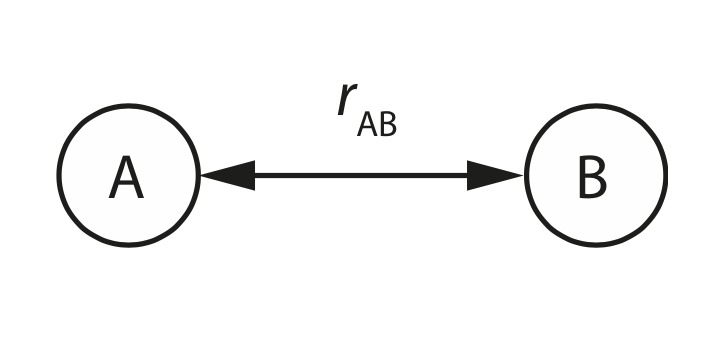
\includegraphics[width=0.9\linewidth]{fig/diatomic_molecule.png}
        \caption{กำหนดระยะห่างระหว่างอะตอม}
        \label{fig:diatomic_mol}
    \end{subfigure}%
    \begin{subfigure}{0.5\textwidth}
        \centering
        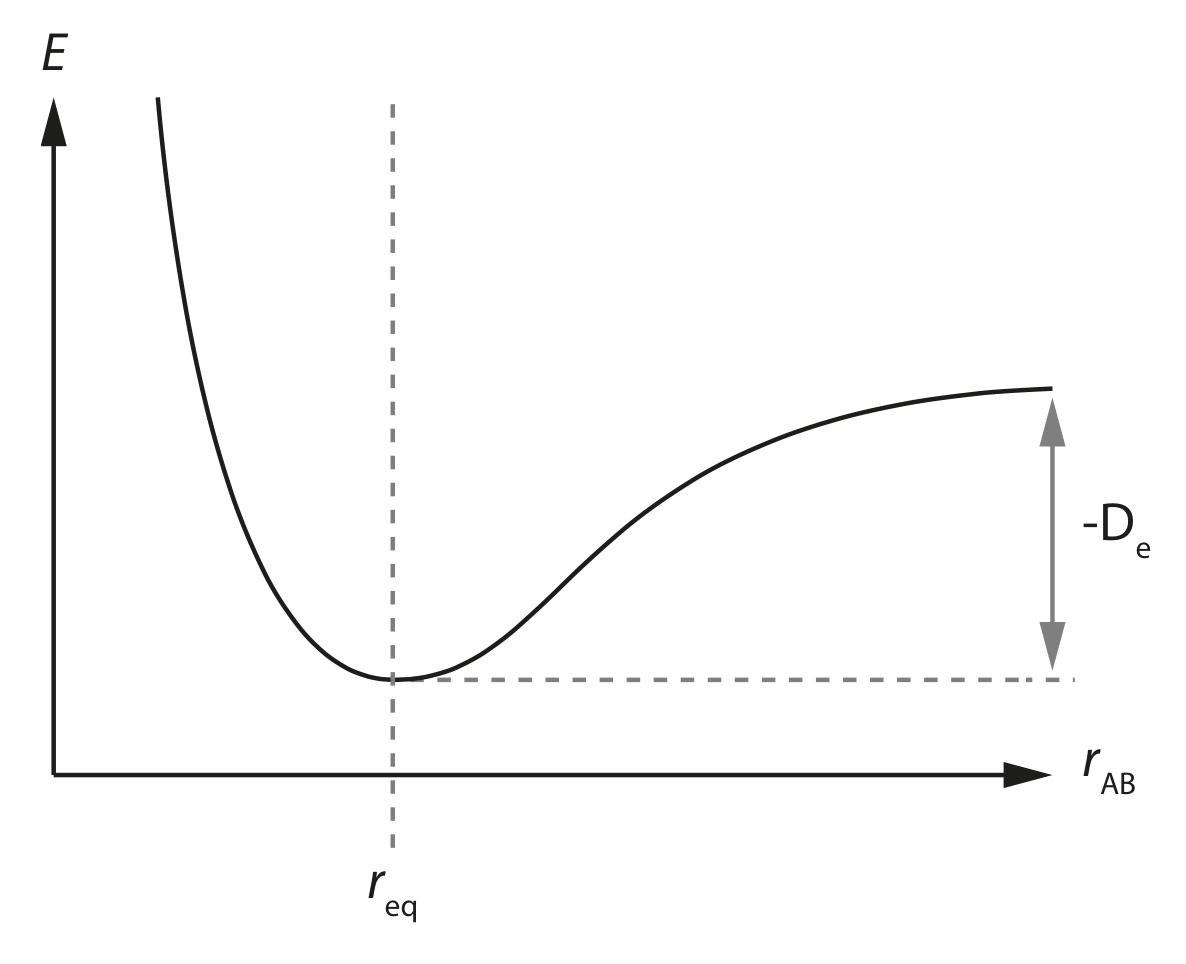
\includegraphics[width=0.9\linewidth]{fig/PES_diatomic_mol.png}
        \caption{พลังงานศักย์ของโมเลกุลคู่}
        \label{fig:PES_diatomic}
    \end{subfigure}
    \caption{โมเลกุลคู่}
    \label{fig:diatomic_mol_and_PES}
\end{figure}

สำหรับคู่อะตอม A และ B มี Degree of Freedom เพียงแค่ 1 Degree เท่านั้น และกำหนดให้ระยะห่างระหว่างอะตอมเป็น $r_{AB}$ ถ้าอะตอม 
A มีการสร้างพันธะกับอะตอม B สิ่งที่เกิดขึ้นคือเรา(อาจจะ)สามารถทำนายลักษณะของ PES ของโมเลกุลนี้ได้ ดังต่อไปนี้

\begin{figure}[htbp]
    \centering
    \begin{subfigure}{0.7\textwidth}
        \centering
        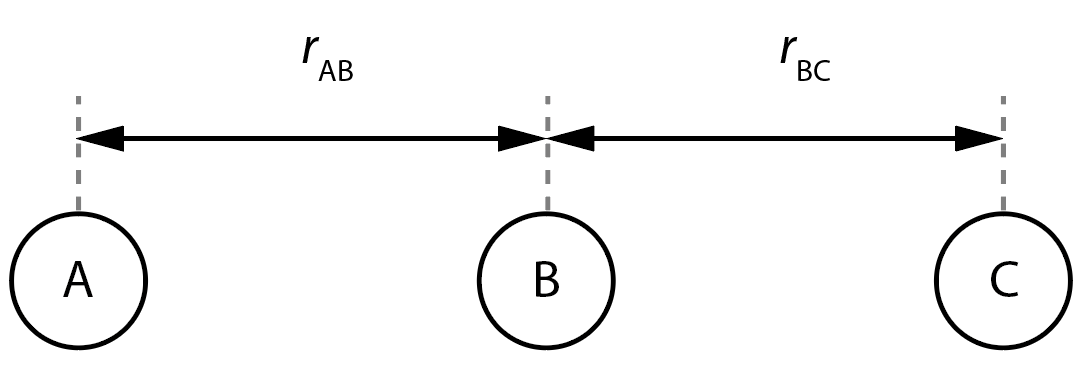
\includegraphics[width=0.9\linewidth]{fig/3-body_collinear.png}
        \caption{กำหนดระยะห่างระหว่างอะตอม}
        \label{fig:3_body_mol}
    \end{subfigure}%
    \\
    \begin{subfigure}{0.9\textwidth}
        \centering
        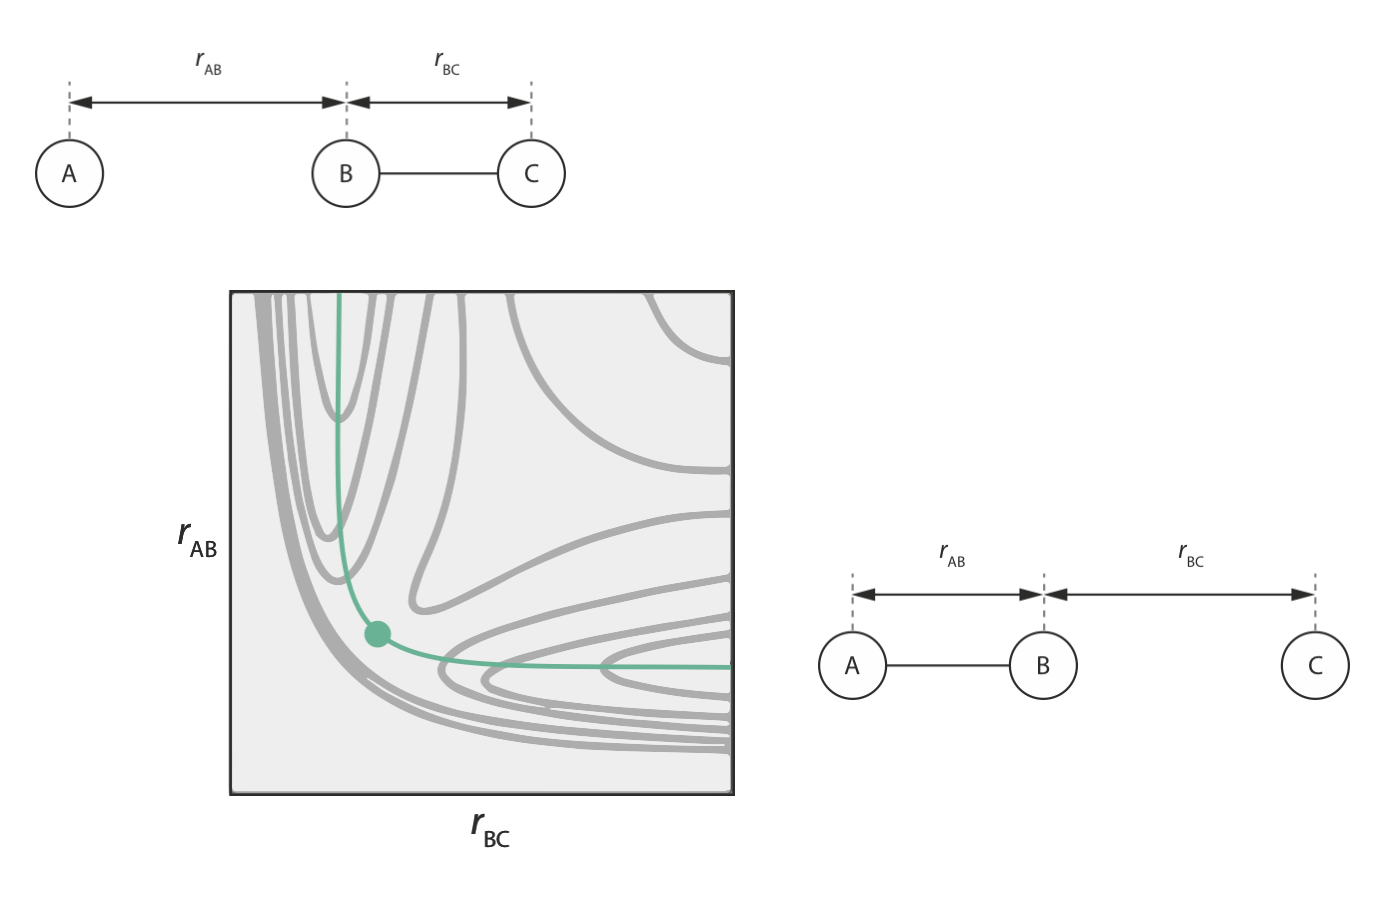
\includegraphics[width=0.9\linewidth]{fig/3-body_collinear_PES.png}
        \caption{พลังงานศักย์ของโมเลกุลสามอะตอมแบบเชิงเส้นตรงร่วม}
        \label{fig:PES_3_body_mol}
    \end{subfigure}
    \label{fig:3_body_mol_and_PES}
\end{figure}

\begin{figure}[htbp]
    \centering
    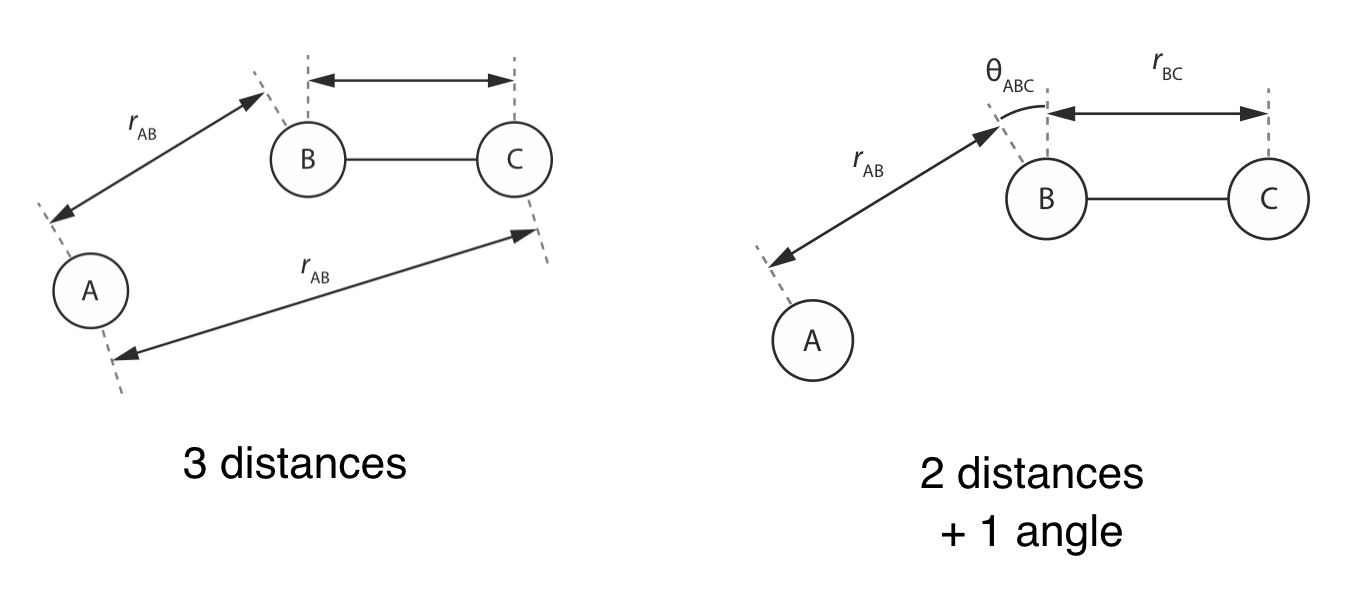
\includegraphics[width=0.9\linewidth]{fig/3-body_non-collinear.png}
    \caption{โมเลกุลสามอะตอมแบบไม่เป็นเชิงเส้นตรงร่วม}
    \label{fig:non_collinear}
\end{figure}

\begin{figure}[htbp]
    \centering
    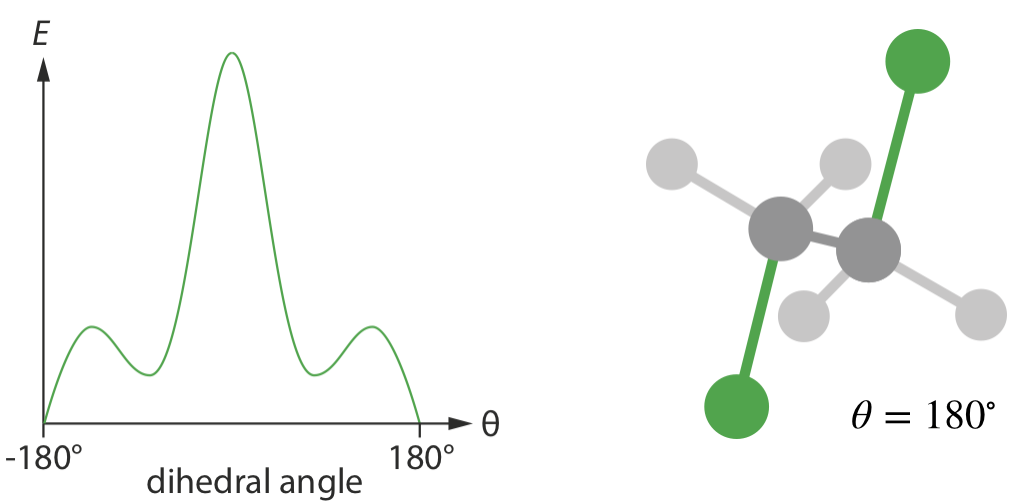
\includegraphics[width=0.9\linewidth]{fig/PES_C2H4Cl2.png}
    \caption{พลังงานศักย์ของโมเลกุล \ce{C22H4Cl2}}
    \label{fig:pes_c2h4cl2}
\end{figure}

%--------------------------
\section{ไดโพลโมเมนต์}
\label{sec:dipole_moment}
\idxboth{ไดโพลโมเมนต์}{Dipole Moment}
%--------------------------

ไดโพลโมเมนต์ (Dipole Moment) คือสภาพมีขั้วไฟฟ้าที่เกิดขึ้นจากการที่กลุ่มของอิเล็กตรอนในโมเลกุลนั้นมีการกระจายตัวที่ไม่สมํ่าเสมอ 
โดยบริเวณที่มีอิเล็กตรอนหนาแน่นมากกว่าจะประพฤติตัวเป็นขั้วลบ ส่วนบริเวณที่มีความหนาแน่นอิเล็กตรอนน้อยกว่าจะประพฤติตัวเป็นขั้วบวก 
ซึ่งมักจะอยู่ทางด้านเดียวกับนิวเคลียสด้วย โดยขั้วไฟฟ้าทั้งสองนี้จะอยู่ด้วยกันเป็นคู่ ๆ และอยู่ตรงข้ามกันเสมอ

ตามธรรมชาตินั้นประจุไฟฟ้าที่วางอยู่ในสนามไฟฟ้าจะถูกออกแรงกระทำทั้งในรูปของแรงผลักและแรงดูดซึ่งขึ้นอยู่กับชนิดของประจุไฟฟ้า กล่าวคือ%
สนามไฟฟ้าออกแรงผลักแก่ประจุไฟฟ้าบวกและออกแรงดึงดูดแก่ประจุไฟฟ้าลบให้เคลื่อนที่ตามแนวของเส้นสนามไฟฟ้า และสําหรับไดโพลโมเมนต์%
เมื่อวางอยู่ในสนามไฟฟ้าก็จะถูกสนามไฟฟ้านี้เหวี่ยงด้วยแรงบิดหรือทอร์กทําให้ขั้วไฟฟ้าทั้งสองของอะตอมเรียงตัวใหม่ หากสนามไฟฟ้ามีลักษณะเอกรูป 
(Uniform) หรือมีความสม่ำเสมอ แรงลัพธ์ทางไฟฟ้าที่เกิดขึ้นต่อประจุทั้งสองจะทําให้ไดโพลโมเมนต์นี้เคลื่อนที่ด้วยความเร่งออกไปตามเส้นของ%
สนามไฟฟ้าต่อไปอย่างช้า ๆ ได้บ้างถ้าหากเป็นไดโพลโมเมนต์ของอะตอมอิสระ

%--------------------------
\section{สภาพการเกิดขั้ว}
\label{sec:polariz}
\idxboth{สภาพการเกิดขั้ว}{Polarizability}
%--------------------------

สภาพการเกิดขั้ว (Polarizability)

%--------------------------
\section{เทคนิคสเปกโทรสโกปีแบบสั่น}
\label{sec:spectro}
\idxen{Spectroscopy}
\idxen{Spectroscopy!Vibrational Spectroscopy}
%--------------------------

สเปกโทรสโกปี (Spectroscopy) เป็นการศึกษาอันตรกิริยา (Interaction) ระหว่างสสารกับรังสีแม่เหล็กไฟฟ้า (Electromagnetic Radiation) 
ที่เกิดจากการเปลี่ยนระดับพลังงานของอิเล็คตรอน การเปลี่ยนระดับพลังงานการหมุน (Rotation) และการสั่นสะเทือน (Vibration) ของโมเลกุล 
ซึ่งการที่เราทราบจากสเปกตรัมของโมเลกุลจะทำให้เราทราบข้อมูลหลายอย่างเกี่ยวกับโครงสร้างของโมเลกุลของสสารและสมบัติทางเคมี เช่น

\begin{itemize}
    \item สมมาตรของโมเลกุล (Symmetry)
    
    \item ความยาวพันธะ (Bond Length)
    
    \item มุมพันธะ (Bond Angle)
    
    \item ความแข็งแรงของพันธะ (Bond Strength)
    
    \item การเปลี่ยนแปลงภายในโมเลกุล
    
    \item การเปลี่ยนแปลงระหว่างโมเลกุล
\end{itemize}

โดยในหัวข้อนี้เราจะมาดูรายละเอียดเกี่ยวกับการคำนวณความเข้มของการดูดกลืนสำหรับเทคนิค Infrared (IR) และรามาน (Raman) 
ซึ่งทั้งสองเทคนิคนี้ต่างก็เป็นเทคนิคสเปกโทรสโกปีแบบสั่น (Vibrational Spectroscopy) ซึ่งมีการนำมาใช้ในการทำงานวิจัยสำหรับการศึกษา%
คุณสมบัติของโมเลกุลอย่างแพร่หลาย

%--------------------------
\subsection{อินฟราเรดสเปกโทรสโกปี}
\label{ssec:ir_spectro}
\idxboth{สเปกโทรสโกปี!อินฟราเรด}{Spectroscopy!IR}
%--------------------------

อินฟราเรดสเปกโทรสโกปี (IR Spectroscopy) เป็นการวัดการดูดกลืนของการแผ่รังสีของโมเลกุลในช่วงอินฟราเรดซึ่งเกี่ยวข้องกับการเปลี่ยนแปลงของ%
อิเล็กทริกไดโพลโมเมนต์ (Electric Dipole Moment) ของโมเลกุลที่ศึกษา สำหรับการคำนวณความเข้มของการดูดกลืน IR ในรูปแบบของวิธีแบบ
Dynamic นั้นสามารถทำได้โดยใช้สมการ (ความสมพันธ์) ดังต่อไปนี้s\autocite{thomas2013}

\begin{equation}\label{eq:IR_corr}
    I_{IR} (\omega) \propto \int \braket{\bm{\dot{\mu}}(\tau) \bm{\dot{\mu}}(\tau+t)}_{\tau} e^{-i \omega t} dt
\end{equation}

\noindent โดยที่ $\bm{\dot{\mu}}$ คืออนุพันธ์ของไดโพลโมเมนต์เทียบกับเวลา, $\omega$ คือความถี่เชิงการสั่น (Vibrational Frequency),
$\tau$ คือเวลาที่เปลี่ยนแปลงไปอย่างช้า ๆ และ $t$ คือเวลาสำหรับการทำ Integration นอกจากนี้ยังจะสังเกตได้ว่าจะมีเทอม
$\braket{\bm{\dot{\mu}}(\tau) \bm{\dot{\mu}}(\tau+t)}_{\tau}$ ซึ่งจะเป็นตัวที่บ่งบอกถึงสหสัมพันธ์ของเวลา (Time Correlation) 
ของ $\bm{\dot{\mu}}$ 

สำหรับกรณีที่เป็นแบบ Static นั้น สเปกตรัมของ IR สามารถคำนวณได้ผ่านอนุพันธ์ของไดโพลโมเมนต์เทียบกับพิกัดหรือตำแหน่งของโหมดการสั่น%
แบบปกติ (Normal Coordinates) ซึ่งจะไม่ขึ้นกับเวลา ด้วยสมการดังต่อไปนี้

\begin{equation}\label{eq:mu_qm}
    \bm{\mu}= \sum_{\mu\nu} P_{\mu\nu} \braket{\phi_{\mu}|\bm{r}|\phi_{\nu}}
\end{equation}

\begin{equation}\label{eq:mu_classical}
    \bm{\mu}=\sum_{J} q_J \bm{R_J}
\end{equation}

โดยที่สมการ \ref{eq:mu_qm} จะเป็นสำหรับกรณีแบบควอนตัมซึ่งจะคำนวณผ่านเมทริกซ์ความหนาแน่นและ Basis Function แต่สมการ 
\ref{eq:mu_classical} จะเป็นสำหรับกรณีแบบดั้งเดิมซึ่งจะคำนวณผ่านจุดประจุ (Point Charge) และพิกัดคาร์ทีเซียนของอะตอม

%--------------------------
\subsection{รามานสเปกโทรสโกปี}
\label{ssec:raman_spectro}
\idxboth{สเปกโทรสโกปี!รามาน}{Spectroscopy!Raman}
%--------------------------

รามานสเปกโทรสโกปี (Raman Spectroscopy) เป็นเทคนิคหนึ่งที่เปรียบเสมือนเป็นพี่น้องกับเทคนิคอินฟราเรดสเปกโทรสโกปี โดยที่ Raman 
Spectroscopy จะเป็นผลมาจากการเกิดการกระเจิงของแสงแบบไม่ยืดหยุ่นในช่วงอินฟราเรด (Infraref), วิสิเบิล (Visible), และอัลตราไวโอเล็ต 
(Ultraviolet) ซึ่งเกี่ยวข้องกับการเปลี่ยนแปลงสภาพการเกิดขั้ว (Polarizability) แบบอิเล็กทริกไดโพล-อิเล็กทริกไดโพล 
(Electric-dipole--electric-dipole) ของสสาร โดยความเข้มของการกระเจิงแบบรามาน $(I_{Raman})$ สามารถคำนวณได้ด้วยความ%
สัมพันธ์ดังต่อไปนี้\autocite{thomas2013}

\begin{equation}\label{eq:Raman_corr}
    I_{Raman} (\omega) \propto \frac{(\omega_{in}-\omega)^4}{\omega} 
    \frac{1}{1-\exp(-\frac{\hbar\omega}{k_{B}T})}S(a^{2}, \gamma^{2})
\end{equation}

\noindent โดยที่ $S(a^{2}, \gamma^{2})$ คือตัวแปรที่เป็นผลจากการรวมกันของความคงที่ (ไม่เปลี่ยนแปลง) แบบไอโซโทรปิค (Isotropic) 
และแอนิโซโทรปิค (Anisotropic)\footnote{คำจำกัดความ: คุณสมบัติที่เท่ากันทุกทิศทาง (Isotropic) และคุณสมบัติที่ขึ้นอยู่กับทิศทาง 
(Anisotropic)} ของเทนเซอร์แบบ Placzek-type Polarizability $(\bm{\alpha})$\autocite{jensen2005}, $\omega$ 
คือความถี่เชิงการสั่น, $\omega_{in}$ คือความถี่ของแสดง, $k_{B}$ คือค่าคงที่ของโบลทซ์มานน์ (Boltzmann Constant) และ $T$ 
คืออุณหภูมิของระบบในหน่วย Kelvin โดยสมการที่จะใช้ในการอธิบาย $S(a^{2}, \gamma^{2})$ จะขึ้นอยู่กับรูปแบบของการทดลองและสมการของ 
Time Correlation\autocite{mattiat2021}

%--------------------------
\section{การถ่ายโอนอิเล็กตรอน}
\label{sec:et}
\idxboth{การถ่ายโอนอิเล็กตรอน}{Electron Transfer}
%--------------------------

การถ่ายโอนอิเล็กตรอน (Electron Transfer) เป็นกระบวนการที่อิเล็กตรอนเปลี่ยนตำแหน่งหรือเคลื่อนย้ายจากอะตอมหนึ่งไปยังอีกอะตอมหนึ่ง 
(Transfering) โดยเราสามารถแบ่งการถ่ายโอนอิเล็กตรอนออกได้เป็นสองกรณีคือการถ่ายโอนระหว่างโมเลกุล (Intermolecular Electron 
Transfer) และการถ่ายโอนภายในโมเลกุล (Intramolecular Electron Transfer) สำหรับการถ่ายโอนกรณีแรกนั้นมีสิ่งเร้าภายนอกเป็นปัจจัยหลัก 
ตัวทำละลายหรือสิ่งแวดล้อมภายนอกเป็นตัวกระตุ้นหรือตัวขับเคลื่อน (Driving Force) ที่ทำให้เกิดการถ่ายโอนจากโมเลกุลหนึ่งไปยังโมเลกุลหนึ่ง
สำหรับการถ่ายโอนกรณีที่สองนั้นจริง ๆ แล้วมีปัจจัยหลายอย่างที่ทำให้เกิดกระบวนการนี้ เช่น ความเสถียรเชิงโครงสร้างของโมเลกุล (Stability) 
ซึ่งเกิดจากการรบกวนจากภายนอกที่ส่งผลให้โครงสร้างเชิงอิเล็กทรอนิกส์ของโมเลกุลเปลี่ยนไป 
\idxth{การถ่ายโอนอิเล็กตรอน!การถ่ายโอนระหว่างโมเลกุล}
\idxth{การถ่ายโอนอิเล็กตรอน!การถ่ายโอนภายในโมเลกุล}
\idxen{Electron Transfer!Intermolecular Transfer}
\idxen{Electron Transfer!Intramolecular Transfer}

ในการพิจารณาการถ่ายโอนอิเล็กตรอนทั้งสองกรณีนั้นสามารถอธิบายได้ดังนี้ ให้ผู้อ่านลองจินตนาการโดยสมมติว่ามีกล่องอยู่สองกล่อง โดยกล่องซ้ายใส่%
ลูกบอลไว้ ส่วนกล่องขวานั้นว่างเปล่า หลังจากนั้นเราทำการหยิบลูกบอลจากกล่องซ้ายแล้วนำไปใส่ไว้ในกล่องขวา ซึ่งนี่คือการจำลองการถ่ายโอนอิเล็กตรอน 
จากเหตุการณ์ดังกล่าวเราแบ่งออกได้เป็นสองเหตุการณ์ย่อยคือ

\begin{enumerate}
    \item เหตุการณ์ที่เกิดขึ้นก่อนที่จะเกิดการถ่ายโอนอิเล็กตรอน
    
    \item เหตุการณ์ที่เกิดหลังจากถ่ายโอนอิเล็กตรอนแล้ว
\end{enumerate}

\begin{figure}[htbp]
    \centering
    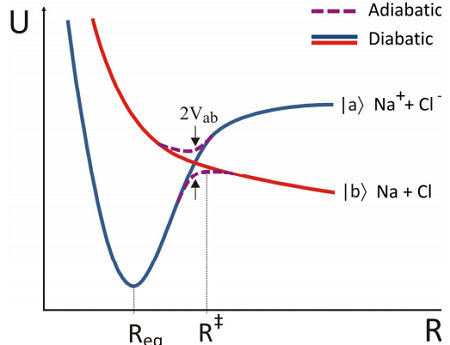
\includegraphics[width=0.7\linewidth]{fig/et_diagram.png}
    \caption{แผนภาพแสดงพื้นผิวพลังงานศักย์ของกระบวนการถ่ายโอนอิเล็กตรอน (เครดิตภาพ: \url{https://chem.libretexts.org})}
    \label{fig:et_diagram}
\end{figure}

%--------------------------
\subsection{ค่าคู่ควบของการถ่ายโอนอิเล็กตรอน}
\label{ssec:et_coupling}
\idxth{การถ่ายโอนอิเล็กตรอน!ค่าคู่ควบ}
\idxen{Electron Transfer!Electron Transfer Coupling}
%--------------------------

ค่าคู่ควบของการถ่ายโอนอิเล็กตรอน (Electron Transfer Coupling) เป็นค่าคู่ควบที่เกิดขึ้นจากการถ่ายโอนอิเล็กตรอน

%--------------------------
\subsection{พลังงานการปรับเปลี่ยนโครงสร้าง}
\label{ssec:reor_ener}
\idxth{พลังงานการปรับเปลี่ยนโครงสร้าง}
\idxen{Reorganization Energy}
%--------------------------

พลังงานการปรับเปลี่ยนโครงสร้าง (Reorganization Energy) คือพลังงาน(ที่น้อยที่สุด)ที่ใช้ในการปรับเปลี่ยนโครงสร้างของโมเลกุลเพื่อทำให้เกิด%
การถ่ายโอนอิเล็กตรอนได้

%--------------------------
\section{คุณสมบัติของสถานะกระตุ้น}
\label{sec:ex_prop}
\idxth{สถานะกระตุ้น}
\idxen{Excited State}
%--------------------------

คุณสมบัติของอิเล็กตรอน ณ สถานะกระตุ้น (Excited State Properties)
\idxth{สถานะกระตุ้น!คุณสมบัติของอิเล็กตรอน ณ สถานะกระตุ้น}
\idxen{Excited State Properties}

%--------------------------
\subsection{พลังงานของสถานะกระตุ้น}
\label{ssec:ex_ener}
\idxth{สถานะกระตุ้น!พลังงานของสถานะกระตุ้น}
\idxen{Excited State!Excited State Energies}
%--------------------------

พลังงานของสถานะกระตุ้น (Excited State Energies)

%--------------------------
\subsection{ค่าคู่ควบของกระบวนการนอนอะเดียแบติก}
\label{ssec:nonadia_ener}
\idxth{สถานะกระตุ้น!ค่าคู่ควบแบบนอนอะเดียแบติก}
\idxen{Excited State!Nonadiabatic Coupling}
%--------------------------

ค่าคู่ควบแบบนอนอะเดียแบติก (Nonadiabatic Coupling)

%--------------------------
\section{การคำนวณโครงสร้างเชิงอิเล็กทรอนิกส์ของโมเลกุล}
\label{sec:comp_elec_strct}
\idxth{โครงสร้างเชิงอิเล็กทรอนิกส์!การคำนวณ}
\idxen{Electronic Structure!Calculation}
%--------------------------

ในหัวข้อนี้เราจะมาดูการคำนวณโครงสร้างเชิงอิเล็กทรอนิกส์ของโมเลกุลกันครับ ซึ่งสิ่งที่เราจะคำนวณนั้นก็คือคุณสมบัติเชิงอิเล็กทรอนิกส์ของโมเลกุล%
นั่นเอง โดยโปรแกรมเคมีเชิงคำนวณที่ผู้เขียนเลือกมาให้ผู้อ่านศึกษาเพื่อเป็นตัวอย่างนั้นก็คือโปรแกรม PySCF ซึ่งเป็นโปรแกรมที่ติดตั้งและใช้งานได้ง่าย 
มีฟังก์ชันที่หลากหลาย รองรับการคำนวณหลากหลายวิธี โดยผู้อ่านสามารถศึกษารายละเอียดเพิ่มเติมได้ในหัวข้อที่ \ref{sec:software_pyscf}

โค้ดต่อไปนี้เป็นการคำนวณคุณสมบัติเชิงอิเล็กทรอนิกส์ของโมเลกุล \ce{HF}

\begin{lstlisting}[style=MyPython]
import pyscf

mol = pyscf.M(
    atom = 'H 0 0 0; F 0 0 1.1',  # in Angstrom
    basis = '631g(d)',
    symmetry = True,
)

mf = mol.KS()
mf.xc = 'pbe0'
mf.kernel()

# Orbital energies, Mulliken population etc.
mf.analyze()
\end{lstlisting}

\vspace{1em}
\noindent ซึ่งจะได้เอาต์พุตดังต่อไปนี้

\begin{lstlisting}[style=plain]
converged SCF energy = -100.302481944224
Wave-function symmetry = Coov
occupancy for each irrep:     A1  E1x  E1y  E2x  E2y
                                3    1    1    0    0
**** MO energy ****
MO #1 (A1 #1), energy= -24.7448119170483 occ= 2
MO #2 (A1 #2), energy= -1.15590146781068 occ= 2
MO #3 (A1 #3), energy= -0.497762978336231 occ= 2
MO #4 (E1x #1), energy= -0.378844054318716 occ= 2
MO #5 (E1y #1), energy= -0.378844054318716 occ= 2
MO #6 (A1 #4), energy= 0.0180305141394873 occ= 0
MO #7 (A1 #5), energy= 0.718896484194941 occ= 0
MO #8 (E1x #2), energy= 1.21692188697545 occ= 0
MO #9 (E1y #2), energy= 1.21692188697545 occ= 0
MO #10 (A1 #6), energy= 1.31220491703922 occ= 0
MO #11 (A1 #7), energy= 1.62220484001697 occ= 0
MO #12 (E1x #3), energy= 1.84298258830569 occ= 0
MO #13 (E1y #3), energy= 1.84298258830569 occ= 0
MO #14 (E2x #1), energy= 1.89656974390515 occ= 0
MO #15 (E2y #1), energy= 1.8965699570922 occ= 0
MO #16 (A1 #8), energy= 2.33936741542906 occ= 0
    ** Mulliken atomic charges  **
charge of  0H =      0.37993
charge of  1F =     -0.37993
Dipole moment(X, Y, Z, Debye):  0.00000,  0.00000, -2.08373
\end{lstlisting}

\vspace{1em}
โดยสรุปผลการคำนวณได้ดังนี้ โมเลกุล \ce{HF} มีพลังงานเชิงอิเล็กทรอนิกส์ $(E_{\text{HF}} + E_{\text{Exchange}} + 
E_{\text{Correlation}})$ เท่ากับ -100.302481944224 Hartree และมีพลังงานของออร์บิทัลเชิงโมเลกุล (MO) ตามที่แสดงทั้ง 16 ออร์บิทัล
